\chapter{Interacción Persona-Ordenador e Interfaces}
\label{chap:interfaces}
\drop{A} lo largo de la historia la interfaz ha ido evolucionando ofreciendo un amplio abanico de opciones,
especializándose y diversificándose para dar lugar a nuevos modelos de interacción, como son las basadas en soportes móviles, interfaces gráficas, tangibles, de realidad aumentada, las interfaces cooperativas y colaborativas, etc. Todas ellas poseen una serie de ventajas y restricciones a la hora de adaptarse a distintos entornos y situaciones.


\section{Interación Persona-Ordenador}
La Interacción Persona-Ordenador (IPO o HCI: Human Computer Interaction), es la disciplina enfocada al estudio de la interacción realizada entre sistemas computacionales y las personas. El objetivo principal es el de mejorar esta interacción  consiguiendo que los sistemas computacionales sean mas manejables, de manera que la interacción sea lo mas intuitiva posible. 
La ACM\footnote{Association for Computing Machinery.} define IPO como: “La disciplina encargada del diseño, evaluación e implementación de sistemas computacionales interactivos para uso humano y del estudio de los que rodea”.

El área de investigación de IPO, es aplicada en el mundo empresarial y académico, siendo una de las razones de cambio en el uso de la informática, mejorando los sistemas a medida que se localizaban nuevas necesidades de usuarios. Un ejemplo de ello son las interfaces gráficas de usuario, que revolucionaron y aumentaron las posibilidades de utilización en el uso en computadoras. A día de hoy para el desarrollo de interfaces software es posible hacer uso de bibliotecas y paquetes ya existentes, que facilitan la programación de los desarrolladores. El crecimiento de “World Wide Web (WWW) es el resultado directo de investigaciones IP0.

La evolución de esta disciplina es debido principalmente a factores como:
\begin{itemize}
\item Creatividad humana: factor fundamental que determina que necesidad se desea cubrir, y como sería del diseño de la misma. Ya en los primeros pasos dados en la ciencia de la informática, visionarios realizaron proyecciones imaginarias de como serian las computadoras y que funciones podrían ser capaces de llevar acabo.
\item El estado del arte en la tecnología: a menudo actuá como límite al diseño.
\item El mercado que engloba las computadoras: está directamente en relación con el precio de los elementos y que indice directamente en que usuario utilizará dicho producto y que uso hace de el.
\end{itemize}

Según Shackel \cite{Shackel}, a principios de los años 50, las computadoras tenían como objetivo la investigación, pensadas principalmente para resolver problemas matemáticos y científicos, donde la fiabilidad de los cálculos era primordial. En la década de los 60 y 70 son fabricadas las primeras macro-computadoras dirigidas a profesionales en el tratamiento de datos. Estas máquinas tenían un altos costes de fabricación y tenían poca flexibilidad, ademas de las dificultades a la hora de ser programadas. En los años 70, las mini-computadoras aparecen en el mercado enfocadas a ingenieros y otros profesionales, y donde aún la programación es elevada y compleja. Sobre los años 80 aparecen las computadoras dirigidas a todo tipo de consumidores, donde la usabilidad toma especial importancia, ya que intenta satisfacer las necesidades y requerimientos que demandan los usuarios. Durante la siguiente década, surgen nuevos dispositivos de menor tamaño, donde la usabilidad sigue siendo su principal característica, presentando nuevas dificultades a los profesionales e investigadores de la IPO.

IPO analiza conjuntamente los aspectos que dependen de la computadora y los que son humanos. Dependiendo del punto de vista desde que se realiza el estudio, el enfoque es tratado desde los siguientes contextos:
\begin{itemize}
\item Contexto humano: es completado por ciencias tales como psicología, ciencias cognitivas, de comunicación, de diseño gráfico e industrial, entre otras.
\item Computadoras y maquinaria: comprende los lenguajes de programación, gráficos por computadora, sistemas operativos, y desarrollo de ambientes.
\end{itemize}

En la Figura~\ref{fig:HCI}, se muestran las disciplinas que intervienen en IPO.

\begin{figure}[!h]
\begin{center}
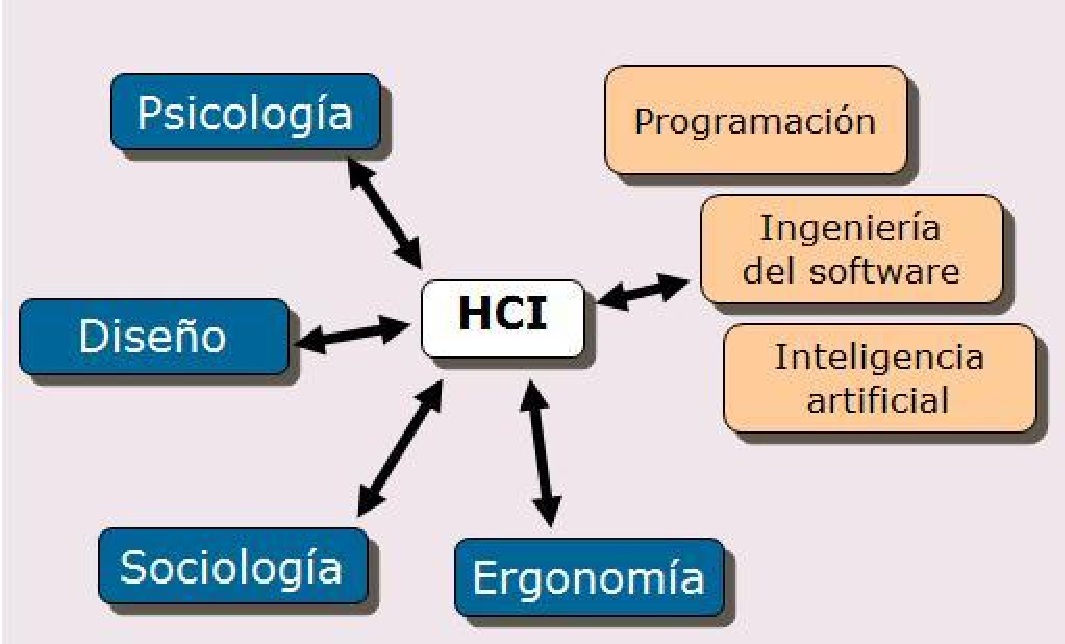
\includegraphics[width=0.5\textwidth]{HCI.pdf}
\caption{Ciencias que se relacionan con el HCI. (Fuente: Interacción tangible en aplicaciones educativas \cite{Artola})}
\label{fig:HCI}
\end{center}
\end{figure}

La interacción entre personas y tecnología se realiza por medio de un componente implícito: la Interfaz.
La perfecta interfaz debe entender las necesidades de los usuarios, sus estilos de interacción natural, apoyándoles para eliminar los problemas en el suso de herramientas computacionales. Para el correcto desarrollo de una interfaz es preciso comprender todos los factores implicados (organizativos, ergonómicos, psicológicos, y sociales), los cuales determinan la manera de actuar de los usuarios y como ellos hacen uso de las computadoras, y conseguir desarrollar herramientas para que los sistemas diseñados satisfagan los requisitos del usuario, y así, conseguir una interacción eficiente, efectiva y segura.


\section{Interfaz Gráfica de Usuario GUI}
La interfaz gráfica de usuario \emph{GUI}\footnote{del inglés, Graphical User Interfaz} hace uso de un conjunto de imágenes y objetos de forma gráfica, para mostrar la información proporcionando un entorno visual sencillo que facilita la interacción “HCI”(Human-Computer Interaction). Algunas de estas GUI son diseñadas para un uso específico como son las pantallas táctiles, que simplifican aún más la interacción HCI mediante el sentido del tacto.
La interfaz entre personas e información digital, requiere de dos componentes fundamentales: la entrada y salida o control y representación. Los controles permiten a los usuarios manipular la información, mientras que las representaciones externas son percibidas por medio de los sentidos humanos. La siguiente representación (ver Figura~\ref{fig:GUI}), muestra el modelo básico de una interacción con interfaz gráficas. En ella se hace uso de un elemento de entrada, como controlador remoto (ratón de ordenador), cuya información digital es procesada para ser representada de manera intangible mediante un monitor o produciendo un sonido determinado. Es decir, el usuario interactúa mediante un dispositivo a distancia y, en última instancia, experimenta una representación intangible de información digital (pixeles y sonido).

\begin{figure}[!h]
\begin{center}
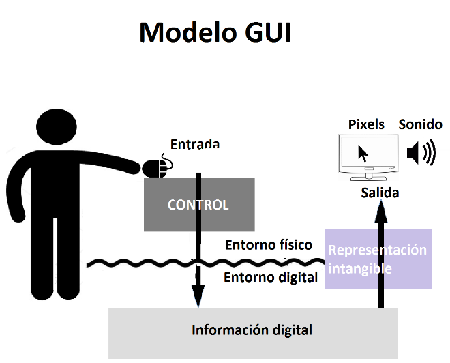
\includegraphics[width=0.5\textwidth]{GUI.pdf}
\caption{Modelo de interacción de las interfaces gráficas (Adaptado de Ishii \cite{Ishii})}
\label{fig:GUI}
\end{center}
\end{figure}

\section{Interfaz Tangible de Usuario TUI}
Las interfaces de usuario tangibles \emph{TUI} (Tangible User Interface), en su área de estudio, tiene como objetivo analizar el paradigma de interacción HCI, no limitándolo a una simple pantalla. Hacer que la información sea comprensible y literalmente captable, es la finalidad principal de la interacción tangible, al proporcionar representación física de los datos digitales mediante objetos que los representen “TUIOs”(Tangible User Interface Objects). Estos objetos pueden ser utilizados con la manipulación natural de los usuarios, realizando un puente de unión entre el mundo digital y el mundo real.

El objetivo detrás de las interfaces tangibles es permitir la interacción con las computadoras a través de objetos familiares, combinando la experiencia del usuario en el mundo táctil con el poder de la tecnología (Ishii, 1997).
Tal interacción física es básicamente de tipo unidireccional, dirigida desde el usuario al sistema, limitando los posibles patrones de interacción. En otras palabras, el sistema no tiene medios para apoyar activamente la interacción física.
La Figura ~\ref{fig:TUI} ilustra la idea clave de hacer uso de la representación tangible (física y captable) como control.

Esta representación tangible ayuda a superar la barrera entre lo físico y lo digital. En contra del modelo GUI propuesto en la Figura ~\ref{fig:GUI}, que hace uso de un ratón como elemento de control, en este caso se hace uso de un prototipo tangible, que intenta incorporar la información digital en forma física. A través de la manipulación física de las representaciones tangibles, la información digital es alterada, mostrando dichos cambios, bien mediante salida en la representación tangible, como en la salida de la representación intangible.


\begin{figure}[!h]
\begin{center}
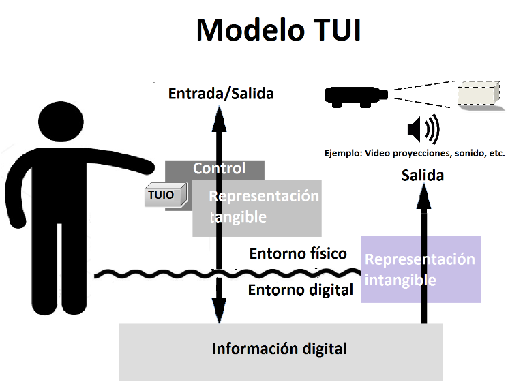
\includegraphics[width=0.5\textwidth]{TUI.pdf}
\caption{Modelo de interacción de las interfaces tangibles (Adaptado de Ishii \cite{Ishii})}
\label{fig:TUI}
\end{center}
\end{figure}


Aunque la representación tangible permite que la realización física se acople directamente a la información digital, tiene capacidad limitada para representar el cambio de muchas propiedades materiales o físicas. A diferencia de los píxeles en la pantalla del ordenador, es muy difícil cambiar un objeto físico en su forma, posición o propiedades (por ejemplo, color, tamaño) en tiempo real. Para complementar esta limitación, TUI también utiliza representaciones tales como proyecciones de video y sonidos para acompañar las representaciones tangibles en el mismo espacio, para dar expresión dinámica de la información digital subyacente.
El éxito de una TUI a menudo se basa en un equilibrio y fuerte acoplamiento perceptual entre las
representaciones tangibles e intangibles. Tanto las representaciones tangibles e intangibles se acoplan perceptualmente para lograr una interfaz transparente que media activamente la interacción con la información digital y borre, de manera apropiada, el límite entre lo físico y lo digital. La coincidencia de entrada y salida junto con una respuesta en tiempo real, son requisitos importantes para lograr este objetivo.

\subsection{Uso de TUI en la educación}

Los sistemas tangibles se están convirtiendo en una alternativa a la interfaz gráfica de usuario. Diferentes marcos de diseño se han aplicado al desarrollo de estos sistemas, abriendo la puerta a nuevas formas de relacionarse con el aprendizaje \cite{Marshall}.

Un diseño tangible, ofrece libertad para poder explorar y manipular objetos físicos y observar que efectos producen sobre el mundo digital. La teoría del aprendizaje y la cognición justifica la asimilación de los conceptos teóricos donde se incluyen las practicas de participación, construcción de modelos, y la actividad colaborativa entre otros. El aprendizaje realizado por medio de elementos tangibles tiene el potencial de que los niños pueden combinar lo conocido y familiar, en nuevas formas \cite{Manches}.

En el área del calculo y sus conceptos abstractos (en los primeros años de educación de los niños), existen varios argumentos acerca de los beneficios de la manipulación de elementos tangibles. Ésta manipulación de elementos físicos, donde interviene la memoria visual, podrían guiar a la resolución de problemas. Investigaciones neurocientíficas, sugieren, que las zonas neuronales activadas durante el proceso de conteo con los dedos de la mano (estrategia de desarrollo seguida por los niños para el aprendizaje de las operaciones de cálculo), con el tiempo ayudan a mejorar las habilidades de manipulación numéricas cuando se es adulto. 

Este hecho pone de manifiesto, que los niños pequeños pueden llegan a reconocer ciertas cosas sin ser capaces de expresare a través del lenguaje, o sin ser capaces de reflexionar sobre lo que pueden llegar a conocer en un sentido explícito \cite{Malley}.


\section{Interfaces Sistema Multi-Pantalla}
Un sistema multi-pantalla o multi-monitor, consiste en combinar varios dispositivos de visualización con el fin de aumentar el espacio visual disponible para ejecutar una o varias tareas.
Inicialmente este tipo de interfaz, fue diseñada con el propósito de mostrar la misma imagen en los distintos dispositivos conectados. Este tipo de uso era aplicado principalmente en las presentaciones, donde el usuario podría disponer de un duplicado de la imagen proyectada.

De manera posterior, los fabricantes aprovecharon esta tecnología para ampliar las aplicaciones posibles, incorporando visualizaciones independientes, aumentando el rango de visión de las aplicaciones, etc.

Son muy distintos los ámbitos de aplicación de esta tecnología, pudiéndose incorporar en los sistemas de control en la industria, sistemas de video-vigilancia, fabricación de juegos, etc.
El uso de varias pantallas en la industria de los videojuegos fue introducida por Nintendo en 1980 con su serie de consolas portátiles \emph{Game and Watch}.


\section{Pantallas capacitivas.}
La gran mayoría de los dispositivos comercialmente disponibles actualmente y que hacen uso de una pantalla, usan la tecnología de contacto capacitivo.
Las pantallas capacitivas multitáctiles no han sido diseñadas para detectar objetos pasivos al ser situados sobre ellas, estas pantallas incluso disponen de filtros para rechazar de manera activa ese tipo de eventos táctiles.
Los \emph{widgets tangibles} en tales pantallas táctiles capacitivas, se han empezado a explorar relativamente hace poco más de una década\cite{Rekimoto}, pero necesitan generalmente del cuerpo del usuario para proporcionar la capacitancia necesaria para la detección del tacto. La gran limitación es que, para mantener la detección, el usuario tiene que seguir tocando la superficie conductora del \emph{widget}.

Las pantallas táctiles capacitivas, detectan la presencia de un conductor eléctrico conectado a tierra, por lo general un dedo humano, cerca de la superficie de la pantalla que es detectado mediante el uso de electrodos transparentes situados encima de la misma.
Principalmente existen dos técnicas de detección: auto capacitancia y capacitancia mutua~\cite{Barrett}. La capacitancia mutua es el método más comúnmente utilizado en pantallas de tipo multitáctil.
La configuración en la que se disponen los electrodos en una pantalla de capacitancia mutua consiste en un conjunto de filas y otro conjunto de columnas. Uno de los conjuntos actúa como transmisores (Tx) y el otro conjunto como receptores (Rx)~\cite{Rekimoto}.

Al aplicar una señal a uno de los electrodos Tx, la capacitancia entre ese electrodo Tx y otro electrodo Rx (que está entrecruzado) acopla la señal al electrodo Rx~\cite{Silicon}. La señal de cada uno de los electrodos Rx es medida y mediante un controlador táctil es determinada la capacitancia entre el electrodo Tx activo y cada uno de los electrodos Rx. Al ser activado un electrodo Tx de manera simultánea (multiplexación en el tiempo), el controlador táctil es capaz de medir esta capacitancia en cada una de las intersecciones de los electrodos Tx - Rx en la pantalla.
Cuando un conductor conectado a tierra como es el caso de un dedo, se aproxima a una de estas intersecciones entre electrodos Tx-Rx, la capacitancia entre ambos electrodos se ve reducida cuando el campo eléctrico entre ellos es perturbado por el conductor~\cite{Zimmerman}.

El paso típico de un electrodo es de 5mm, al realizar un toque sobre la pantalla se verán afectadas mas de una intersección. El controlador táctil mediante interpolación es capaz de determinar el centro del área tocada e informa de ello con un evento táctil.

La mayor parte de los controladores están diseñados para detectar toques con los dedos, aceptando formas elípticas del tamaño de la yema del dedo y rechazando e ignorando eventos táctiles con otras formas y tamaños que pueden reportar eventos táctiles impredecibles.

Resumiendo, para que el controlador informe de un evento táctil, la capacitancia del electrodo Tx-Rx ha de ser reducida por debajo de cierto umbral y ha de suceder a lo largo una elíptica que forma la yema de un dedo.


\subsection{Funcionamiento de un \emph{widget capacitivo}.}

Se define \emph{widget capacitivo} como un objeto tangible completo que contiene uno o más marcadores en su parte inferior y que comunican su posición a la superficie táctil de la pantalla capacitiva. Cada marcador consiste en una almohadilla redonda conductiva que es detectada por la superficie de la pantalla.

Un marcador de \emph{widget} para poder ser detectado como evento táctil sobre la superficie de la pantalla capacitiva tiene que cumplir el requisito de conexión a tierra. Esto se puede conseguir mediante la capacitancia corporal de un usuario como propone Rekimoto~\cite{Rekimoto}. Esto requiere que el usuario toque el \emph{widget} y que las almohadillas del mismo sean conductivas, además de estar conectadas eléctricamente a la parte del \emph{widget} que es tocada por el usuario. De esta forma el \emph{widget} funciona simplemente como conductor eléctrico entre usuario y superficie táctil. Este enfoque tiene el inconveniente de tan pronto como el usuario deja de tener contacto, el controlador de la pantalla no puede detectar ninguna variación de capacitancia.

Otro enfoque que permite reemplazar al usuario como tierra eléctrica, es el uso de un cable conductor que conecta permanentemente el \emph{widget} a un objeto relativamente conectado a tierra, como es el conector negativo de una batería.





% Local Variables:
%  coding: utf-8
%  mode: latex
%  mode: flyspell
%  ispell-local-dictionary: "castellano8"
% End:
